\section{Classification Approach Results}

\subsection{Results}
\Cref{tab:able_class_perf,tab:amputee_class_perf} show the overall
classification accuracies, sensitivities, and specificities for the forward and
backwards classifiers for the able-bodied and amputee subjects respectively. The
forward and backwards classifiers for both subjects achieve high specificity
(the number of normal steps classified correctly) and accuracy $(>95\%)$. The
sensitivity, the percentage of true trips classified correctly, of the
classifiers for both subjects is substantially lower than the specificity or
accuracy. For the forward classifier, we see that because the model is trained
online, the sensitivity improves from the first half of the trial to the second
half, which explains some of the low overall sensitivity.

\begin{table}[htb]
\centering
\begin{tabular}{lccc}
    \multirow{2}{*}{Controller} & Classification & \multirow{2}{*}{Sensitivity} &
        \multirow{2}{*}{Specificity}\\
                                & Accuracy       &             &            \\
    \midrule
    Forward, $1^\tn{st}$ Half & 96\% \vsigstarone &  73\% \vsigstartwo & 99\%\\
    Forward, $2^\tn{nd}$ Half & 99\% ~            &  93\% ~            & 99\%\\
    Forward Overall           & 98\% ~            &  85\% \vsigstartwo & 99\%\\
    Backward                  & 99\% ~            & 100\% ~            & 99\%
\end{tabular}
\caption[Classifier Performance, Able-Bodied]{Classifier Performance
\protect\footnotemark, Able-Bodied Steps: 446, Avoidance Attempts:
53}\label{tab:able_class_perf}
\end{table}
\footnotetext{$\star \implies p<0.05$, $\star\star \implies p<0.01$,
$\star\negmedspace\star\negmedspace\star \implies p<0.001$, Chi-squared
test}

\begin{table}[htb]
\centering
\begin{tabular}{@{}lccc@{}}
    \multirow{2}{*}{Controller} & Classification & \multirow{2}{*}{Sensitivity} & 
        \multirow{2}{*}{Specificity} \\
               & Accuracy       &             &             \\
    \midrule
    Forward, $1^\tn{st}$ Half & 95\% & 80\% ~            & 98\%\\
    Forward, $2^\tn{nd}$ Half & 96\% & 85\% ~            & 98\%\\
    Forward Overall           & 95\% & 83\% \vsigstarone & 98\%\\
    Backward                  & 98\% & 90\% ~            & 99\%
\end{tabular}
\caption[Classifier Performance, Amputee]{Classifier Performance, Amputee, Total
Steps\protect\footnotemark[\value{footnote}]: 222, Avoidance Attempts:
40}\label{tab:amputee_class_perf}
\end{table}

Importantly, the ability of the forward classifier to correctly trigger the
bang-bang obstacle avoidance trajectories improves obstacle avoidance success
rates as shown in \cref{tab:success}. Both subjects were able to avoid
significantly more obstacles with the obstacle avoidance controller than with
the minimum jerk trajectory controller.

\begin{table}[htb]
\centering
\begin{tabular}{@{}lcc@{}}
    \multirow{2}{*}{Controller} & Able-Bodied  & Amputee \\
                                & Success Rate & Success Rate\\
    \midrule
    Minimum Jerk       & 37\% \vsigstarthree & 35\% \vsigstarthree\\
    Adaptive Bang-Bang & 89\% ~~             & 71\% ~~\\
\end{tabular}
\caption[Obstacle Avoidance Success Rates]{Obstacle Avoidance Success
Rates\protect\footnotemark[\value{footnote}]}\label{tab:success}
\end{table}

We also compared our online learning approach for obstacle avoidance to an
offline approach similar to that taken by \citet{lawson2010stumble,
zhang2011towards}, and \citet{shirota2015transfemoral}. To do this, we trained a
classifier offline using the first half of the amputee subject's bang-bang
control data and tested it on the second half of the data. \Cref{tab:offline}
shows that the classifier trained offline has trouble generalizing to the second
half of the data, as it performs significantly worse than the online-trained
model in terms of accuracy and sensitivity.

\begin{table}[ht]
\centering
{\begin{tabular}{@{}lccc@{}}
    Classifier & Classification Accuracy & Sensitivity         & Specificity \\
    \midrule
    Offline    & 89\% \vsigstarone       & 39\% \vsigstarthree & 100\% \\
    Online     & 95\% ~                  & 83\% ~              & 98\%\\
\end{tabular}}
\caption[Online and Offline Forward Classifier Performance, Amputee]{Online and
Offline Forward Classifier Performance,
Amputee\protect\footnotemark[\value{footnote}]}\label{tab:offline}
\end{table}

Finally, we examined the ability of the knee angle regression to choose a target
knee angle that is appropriate for the object size. The feedback law proposed in
\cref{eq:tgt_angle} assumes we can use the backwards classifier score as a
metric of obstacle difficulty. For the able-bodied subject, this assumption
seems warranted, as there is a strong relationship between the obstacle height
and the classifier score (\cref{fig:reg_and_height}a, $R^2 = 0.50$). However,
for the amputee subject, who was less experienced with walking with the powered
prosthesis, this relationship is less clear (\cref{fig:reg_and_height}B, $R^2 =
0.22$).

As shown in \cref{fig:reg_and_height}c\&d, our system is able to ensure that
high classification score steps, associated with high user effort, obtain larger
target flexion angles. This relationship led to noisy volitional control of the
knee flexion angle for the able-bodied subject (\cref{fig:reg_and_height}e) as
evidenced by the linear relationship between knee angle and obstacle height
$(R^2 = 0.31)$. However, for the amputee subject, there is no clear relationship
between the obstacle height and knee flexion angle (\cref{fig:reg_and_height}f,
$R^2 = 0.10$). 

\begin{figure*}[tb]
\centering
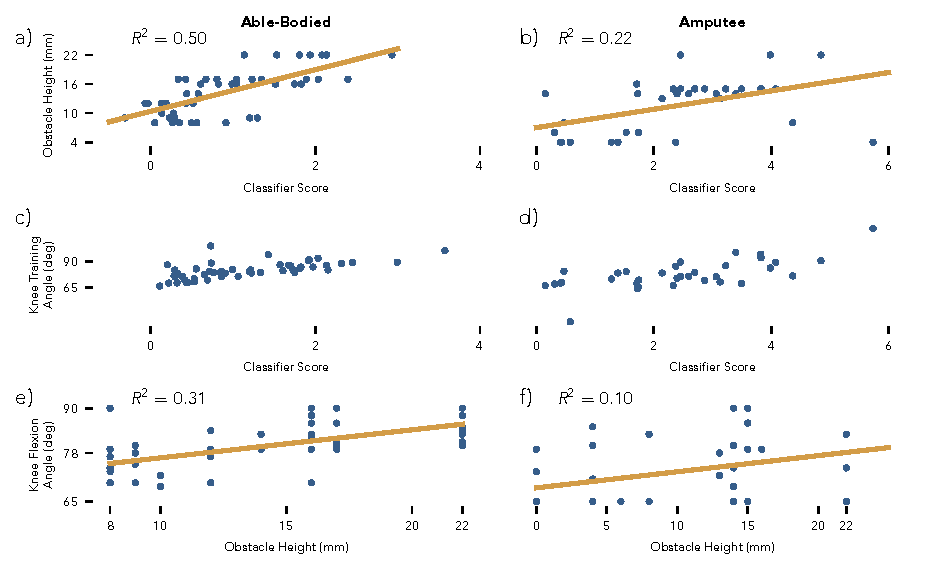
\includegraphics[width=\textwidth]{reg_and_height}
\caption{Obstacle height vs backwards classifier score for (a) the able-bodied
and (b) amputee subjects. The system uses the backwards classifier score as a
metric for obstacle avoidance difficulty. This score is used in a feedback loop
that forms the training set for the flexion target angle regression (c-d). With
this feedback system, the able bodied user (e) is able to achieve a degree of
volitional control over flexion angle as evidenced by the linear relationship
between knee flexion angle and obstacle height $(R^2=0.31)$. However, the
amputee (f) was not able to achieve meaningful control over the flexion of the
prosthesis $(R^2=0.10)$, possibly due to the decreased experience level of this
subject.}\label{fig:reg_and_height}
\end{figure*}
